% -*- root: ../main.tex -*-
%!TEX root = ../main.tex
% this file is called up by main.tex
% content in this file will be fed into the main document
% vim:textwidth=80 fo=cqt

To demonstrate that a suitable advancement of the field has indeed been achieved
through  this system  identification exercise,  a comparison  with the  existing
state of the art in reduced  order electrolyte modelling is warranted. Secondly,
to  comprehend its  extent of  validity  and performance  boundaries, the  newly
developed \gls{rom} must also be  pitted against the full-order \gls{p2d} model.
This section  aims to  provide such  a comparative discussion  for two  types of
inputs ---
\begin{enumerate*}[label=\itshape\alph*\upshape)]
    \item constant current inputs
    \item dynamic load profiles
\end{enumerate*}

\subsection{Constant current inputs}

\Cref{fig:tfquadp2dspatialionicconc1C} shows  the spatial distribution  of ionic
concentration  in  the electrolyte  along  cell  thickness  for a  1C  discharge
beginning at \SI{100}{\percent} \gls{soc}. The spatial concentration computed by
each of the three approaches ---
\begin{enumerate*}[label=\roman*)]
    \item the \gls{p2d} model,
    \item the quadratic approximation model and
    \item the newly developed system identification model(s).
\end{enumerate*}

\begin{figure}[!htbp]
    \centering
    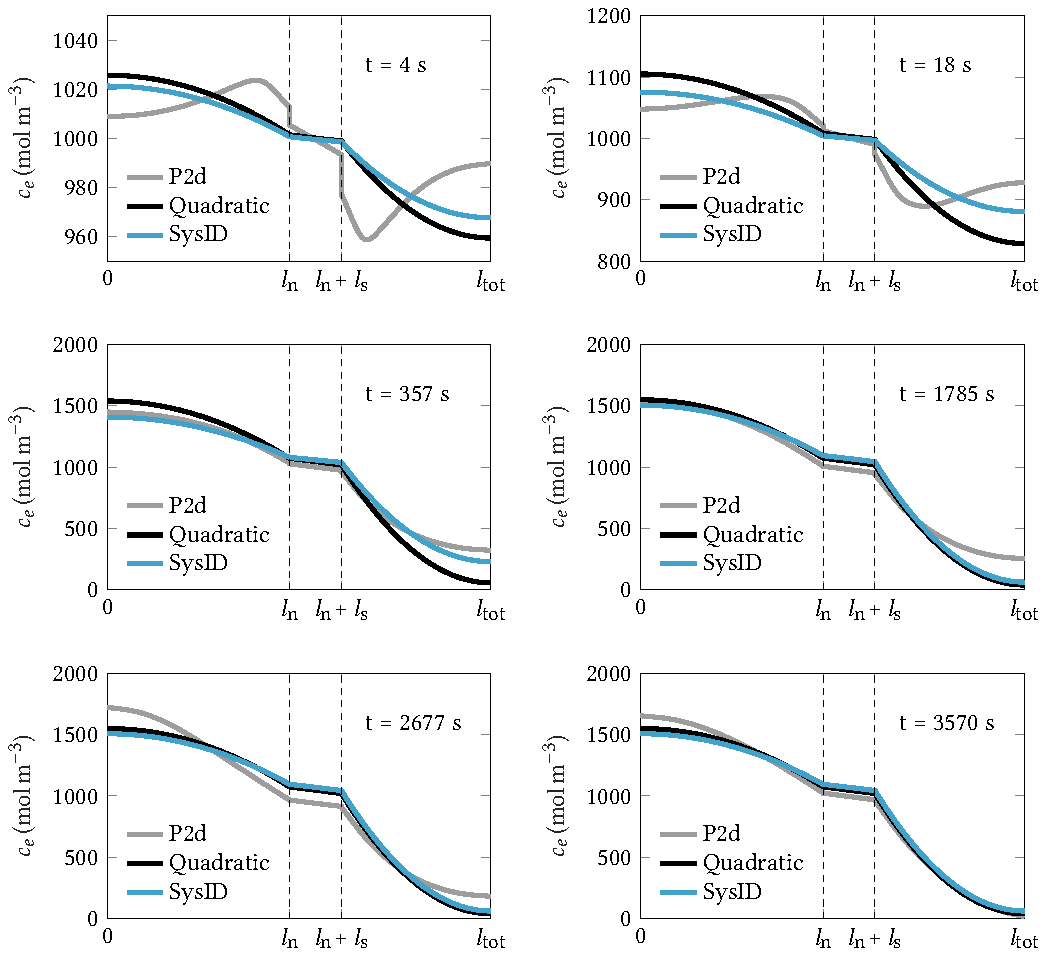
\includegraphics[width=\textwidth]{tf_quadratic_ce_approx_spatial.pdf}
    \caption[Spatial distribution of ionic concentration in
    electrolyte for a 1C discharge computed by the \glsfmtshort{p2d}, quadratic
    approximation \& system identification models]{%
        Spatial distribution of ionic concentration  in electrolyte along cell
        thickness at various  snapshots of  time computed  by each of  the three
        models for  a 1C discharge.  The concentration  profile  computed by
        the  \gls{p2d} model is used as the benchmark reference. The  system
        identification model performs noticeably better than the quadratic
        approximation model during  the initial  transient  while delivering a
        similar performance as a \gls{qss} is reached.
}%
\label{fig:tfquadp2dspatialionicconc1C}
\end{figure}

During  the  initial  phase  of   discharge,  the  \gls{p2d}  model  exhibits  a
characteristic inflection point near the  separator interfaces that diffuses out
over time  until a  \gls{qss}. This  is due to  the fact  the reaction  front is
initially established  close to the  separator, and as surface  concentration of
lithium  in particles  near separator  is  depleted, the  reaction starts  moves
further  into the  electrode thickness.  Neither  of the  two \glspl{rom}  under
consideration here  could successfully  capture this  characteristic inflection.
This is  explained by  the fact  that both  of them  use the  standard quadratic
approximation profile for the \emph{spatial}  profile, which means that only one
apex  point is  possible  per  electrode, which  is  pinned  to their  separator
interfaces by design.

During the transient portion of discharge (approximately up to \SI{357}{\second}
as   shown   in~\cref{fig:tfquadp2dspatialionicconc1C}),   the  locus   of   the
concentration  profile computed  by  the newly  developed system  identification
model(s) clearly lies  much closer to the \gls{p2d} model  than that computed by
the  quadratic  approximation model.  After  the  initial transition  phase,  it
appears  that  the  concentration  profile predicted  by  both  the  \glspl{rom}
converge to the \gls{p2d} model's concentration profile.


To obtain  a quantifiable  perspective on  the accuracy  of the  newly developed
model, it  is desirable  to plot  the temporal  evolution of  the concentration,
particularly  at  the  two  current   collector  interfaces.  The  behaviour  of
the  baseline  quadratic approximation  model  in  this regard  was  established
in~\cref{subsubsec:simresultsbaselinequad}.   Therefore  it   is  important   to
ascertain whether a noteworthy improvement  was achieved using the model arrived
at using the system identification procedure.

\begin{figure}[!htbp]
    \centering
    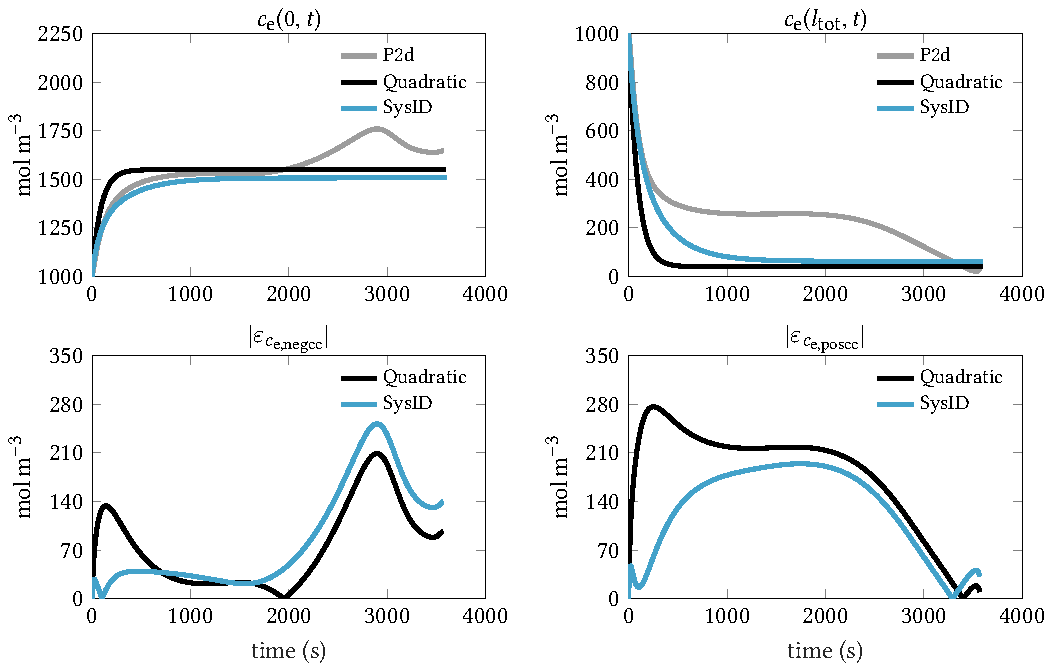
\includegraphics[width=\textwidth]{tf_quad_ce_at_cc_1Cdischg}
    \caption[%
    Time evolution  of ionic  concentrations at  current collectors  computed by
    \glsfmtshort{p2d}, quadratic  approximation \& system  identification models
    for 1C discharge
    ]%
    {%
    Evolution  of ionic  concentration over  time at  the two  current collector
    interfaces for a 1C discharge for
    \begin{enumerate*}[label=\roman*)]
        \item the \glsfmtshort{p2d} model,
        \item the quadratic approximation model and
        \item the newly developed system identification model(s)
    \end{enumerate*}
    (top row). For the quadratic approximation and system identification models,
    the time evolution of their absolute error relative to the \glsfmtshort{p2d}
    benchmark  is also  shown  (bottom  row). At  both  current collectors,  the
    transient performance of the system  identification model is superior to the
    quadratic  approximation model.  At \gls{qss},  the quadratic  approximation
    model is slightly more accurate than the system identification model.
}%
\label{fig:temporalcetfquadratic}
\end{figure}

\Cref{fig:temporalcetfquadratic}   shows  the   time-evolution   of  the   ionic
concentrations at the current collector  interfaces of the negative and positive
electrodes for a 1C discharge. The  concentration profiles computed
by the three approaches ---
\begin{enumerate*}[label=\roman*)]
    \item \glsfmtshort{p2d} model,
    \item quadratic approximation model and the
    \item newly developed system identification model(s)
\end{enumerate*}
are overlaid in the top row of  plots, wherein the left hand side corresponds to
the  current collector  interface  at  the negative  electrode  while the  right
hand  side  corresponds  to  that  at  the  positive  electrode.  The  plots  in
the bottom  row of~\cref{fig:temporalcetfquadratic}  show the  time-evolution of
the  absolute  value  of  their  errors. The  concentration  error  of  each  of
the  two  \glspl{rom}  is  defined  with  respect  to  the  benchmark  \gls{p2d}
model  \ie{}  $\varepsilon_{c_{\text{e,}j}(t)}   =  c_{\text{e,}j_\text{ROM}}  -
c_{\text{e,}j_\text{p2d}}(t)$. The  absolute value  of the  error is  plotted so
that  the magnitude  of the  error can  be visualised  better, aiding  immediate
comparisons based on the plots.

For both  current collectors,  the newly  developed system  identification model
outperforms the  quadratic approximation  model during  the transient  phase. At
the  negative electrode/current  collector interface,  the error  of the  system
identification model remains strictly below  that of the quadratic approximation
model until \approx \SI{650}{\second} and remains comparable to it until \approx
\SI{1600}{\second}. Beyond  this time, the  quadratic approximation model  has a
slightly better accuracy, although the system identification model still remains
at a comparable distance from  it. After \approx \SI{2000}{\second}, both models
yield  the same  response shape.  For the  positive electrode/current  collector
interface, the  error of the system  identification model remains below  that of
the quadratic approximation model until \approx \SI{3300}{\second}.

\begin{figure}[!htbp]
    \centering
    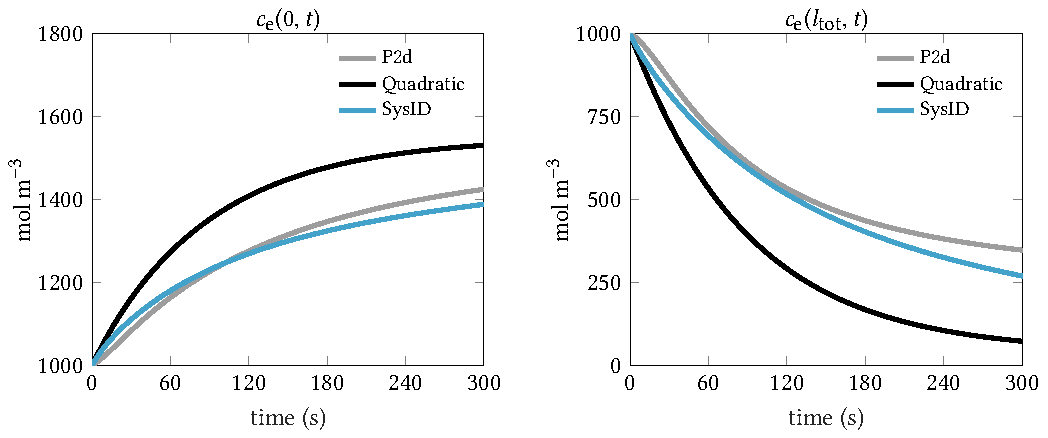
\includegraphics[width=\textwidth]{zoomed_tf_quad_ce_at_cc_1Cdischg.pdf}
    \caption[%
    Transient phase of ionic  concentration evolution at  the two current collectors  computed by
    \glsfmtshort{p2d}, quadratic  \& system  identification models
    for 1C discharge
    ]%
    {%
    Transient phase of the temporal evolution  of ionic  concentration at  the two  current collector
    interfaces for a 1C discharge as computed by ---
    \begin{enumerate*}[label=\roman*)]
        \item the \glsfmtshort{p2d} model,
        \item the quadratic approximation model, and
        \item the newly developed system identification model(s).
    \end{enumerate*}
    The significantly improved accuracy of the system identification model(s)
    relative to the state of the art quadratic approximation model is clearly demonstrated.
}%
\label{fig:zoomedcetfquadtemporal}
\end{figure}

\Cref{fig:zoomedcetfquadtemporal} shows  a zoomed version of  the time-evolution
of the  ionic concentration  at the  two current  collectors, wherein  the first
\SI{300}{\second}  after  application  of  the  load  current  is  plotted.  The
significant  improvement in  accuracy  achieved by  the  newly developed  system
identification model(s) is clearly demonstrated. At both the current collectors,
the concentration computed  by the system identification  model(s) closely track
that of the benchmark \gls{p2d} model.

The  loss  of fidelity  exhibited  past  the  initial transient  phase  warrants
an  explanation. It  should  be  recalled that  the  natural  decoupling of  the
temporal and  spatial systems were taken  advantage of in developing  the system
identification technique. This  means that, for the spatial  profile, the system
identification  model reverts  to the  same  quadratic profile  as the  baseline
quadratic approximation  model. This  explains why the  two models  have similar
shape past the initial transient. During  the transient phase when the \gls{qss}
behaviour is yet to be established, it is reasonable to assume that the temporal
dynamics  are of  paramount importance  in governing  the concentration  profile
evolution.  After a  \gls{qss}  has  been established  with  the reaction  front
diffusing out  and a steady  stream of ion-electron  separation/recombination in
place,  it is  hypothesised  that the  temporal dynamics  have  settled and  the
spatial configuration assumes importance.

With a  sustained application  of constant current  past the  initial transient,
strong spatial gradients  in the ionic concentration are  established within the
cell \ie{} the  concentrations are far from the initial  equilibrium value. This
precisely  exposes the  realm  where the  system  identification model  exhibits
its  natural  weakness.  By  following  the  theory  of  system  identification,
which  necessitates   bias  removal,   the  training  and   validation  profiles
of~\cref{fig:sysidtrainingcurrent}   and~\cref{fig:sysidvalidationcurrent}   had
nearly  zero mean.  This means  that the  currents were  as equally  positive as
negative leading to a small-signal  perturbation around the equilibrium value of
the electrolyte  concentration. While this  profile is ideally suited  to excite
the system's  dynamics, it  fails to  capture the large  signal behaviour.  As a
topic  of future  research,  perhaps a  spatially-coupled system  identification
could be attempted to handle this issue.

The  main  implication of  these  results  is  that  the identified  models  are
primarily suitable for  transient \ie{} dynamic load profiles,  which is typical
of a real-life scenario in an electric/hybrid electric vehicular operation. Such
a  model is  less  suitable  for sustained  constant  current application.  This
implies that  a \gls{bms} in a  vehicle undergoing a \gls{cccv}  charging cannot
rely on  these identified electrolyte  models. However, this exclusion  does not
seriously hamper the model's wider applicability since a simple coulomb-counting
approach with  a high-precision \gls{adc} is  much more accurate than  any other
physics based model in this particular scenario.

Although constant  current discharge is  not a practical use-case  for vehicular
batteries, performing this benchmark evaluation  has helped in understanding the
limits of the newly  developed model. This study has also  helped in providing a
glimpse of its  potential strength \viz{} significantly  improved accuracy under
dynamic load conditions, which is presented next.

\subsection{Dynamic load profiles}


\begin{figure}[!htbp]
    \centering
    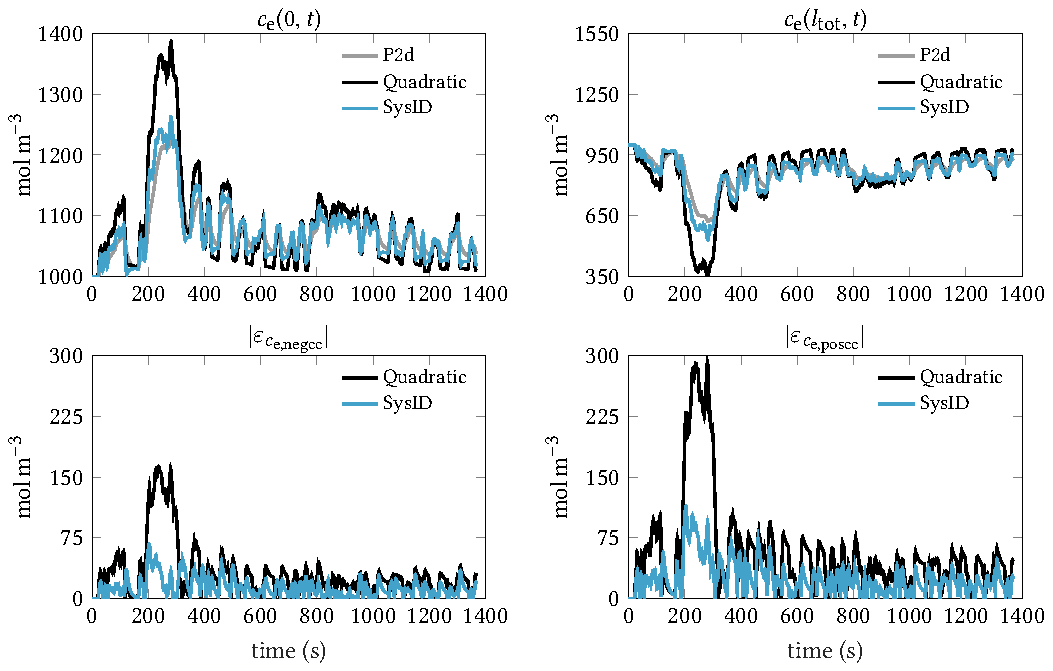
\includegraphics[width=\textwidth]{tf_quad_ce_at_cc_udds}
    \caption{}
    \label{}
\end{figure}

\begin{figure}[!htbp]
    \centering
    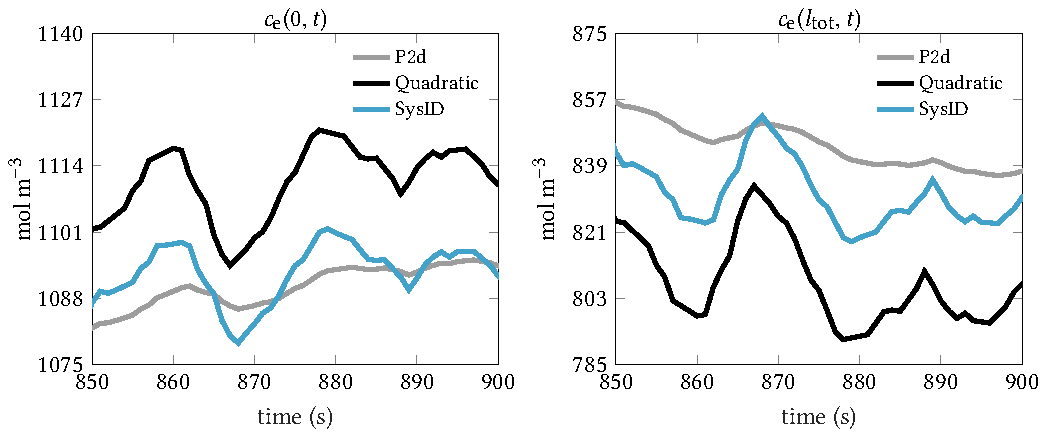
\includegraphics[width=\textwidth]{zoomed_tf_quad_ce_at_cc_udds}
    \caption{}
    \label{}
\end{figure}

